\documentclass[conference]{IEEEtran}
\IEEEoverridecommandlockouts
% The preceding line is only needed to identify funding in the first footnote. If that is unneeded, please comment it out.
\usepackage{cite}
\usepackage{amsmath,amssymb,amsfonts}
\usepackage{algorithmic}
\usepackage{graphicx}
\usepackage{textcomp}
\usepackage{xcolor}
\usepackage{mathtools}
\usepackage{breqn}
\def\BibTeX{{\rm B\kern-.05em{\sc i\kern-.025em b}\kern-.08em
    T\kern-.1667em\lower.7ex\hbox{E}\kern-.125emX}}
\begin{document}

\title{Safety and stability analysis of FollowerStopper\\
%{\footnotesize \textsuperscript{} }
%\thanks{Identify applicable funding agency here. If none, delete this.}
}

\author{\IEEEauthorblockN{Daniel Fishbein}
\IEEEauthorblockA{\textit{Physics, Astronomy, and Materials Science Department} \\
\textit{Missouri State University}\\
Springfield, MO, United States \\
fishbein486@live.missouristate.edu}
\and
\IEEEauthorblockN{Chris Kreienkamp}
\IEEEauthorblockA{\textit{Aerospace and Mechanical Engineering} \\
\textit{University of Notre Dame}\\
Notre Dame, IN, United States \\
ckreienk@nd.edu}
\and
\IEEEauthorblockN{Rahul Bhadani}
\IEEEauthorblockA{\textit{Electrical and Computer Engineering} \\
\textit{University of Arizona}\\
Tucson, AZ, United States \\
rahulbhadani@email.arizona.edu}
\and
\IEEEauthorblockN{Dr. Jonathon Sprinkle}
\IEEEauthorblockA{\textit{Electrical and Computer Engineering} \\
\textit{University of Arizona}\\
Tucson, AZ, United States \\
jsprinkle@email.arizona.edu}
}

\maketitle

\begin{abstract}
In this paper we demonstrate that the velocity controller, FollowerStopper, is safe and string stable. FollowerStopper is a controller that is meant to be implemented on an autonomous vehicle or in an adaptive cruise control (ACC) system. It takes as inputs the autonomous vehicle's velocity, relative distance to the car in front, relative velocity to the car in front, and a desired velocity.  It then commands a new velocity for the autonomous vehicle which will either be the desired velocity or some lower velocity if that is necessary to maintain a safe distance to the car in front. Through mathematical proof, simulation in Simulink, and hardware in the loop implementation on a real autonomous vehicle through Robot Operating System (ROS) and Gazebo, several results are achieved. It is found that, given a maximum LiDAR range of 81 m, there is a maximum permissible safe speed of the car based on its maximum deceleration, and the car is programmed so that it will never be less than 1 m from the vehicle in front. It is shown that a vehicle with FollowerStopper in a singular lane without merges will not crash and that it will be string stable, effectively dissipating human-caused traffic waves if enough vehicles are deployed in the traffic flow.
\end{abstract}



%%%%%%%%%%%%%%%%%%%%%%%%%%%%%%%%%%%%%%%%%%%%%%%%%%%%%%%
%%%%%%%%%%%%%%%%%%%%%%%%%%%%%%%%%%%%%%%%%%%%%%%%%%%%%%%
%%%%%%%%%%%%%%%%%%%%%%%%%%%%%%%%%%%%%%%%%%%%%%%%%%%%%%%



%\begin{IEEEkeywords}
%component, formatting, style, styling, insert
%\end{IEEEkeywords}


%%%%%%%%%%%%%%%%%%%%%%%%%%%%%%%%%%%%%%%%%%%%%%%%%%%%%%%
%%%%%%%%%%%%%%%%%%%%%%%%%%%%%%%%%%%%%%%%%%%%%%%%%%%%%%%
%%%%%%%%%%%%%%%%%%%%%%%%%%%%%%%%%%%%%%%%%%%%%%%%%%%%%%%


\section{Introduction and Related Work}
In order to maintain safety while driving, humans need a certain amount of safe distance between their car and the car directly in front of them so that if the car in front stops abruptly, they can react and stop in time to prevent a crash. From here forward the car which is of interest will be termed the autonomous vehicle (AV) and the car directly in front will be termed the lead vehicle. If the cars are traveling at a slow speed, the AV can follow at a closer distance because the car will not travel as far during the time it takes to react to the lead and to brake.
When the number of cars on a section of highway increases, the car density increases, often termed as congestion. When highways are congested, cars must travel closer together than they normally would, so drivers must drive slower than the speed limit to maintain safety.

It was shown that humans, once the congestion reaches a certain threshold, will inevitably cause traffic jams. This will occur even if there are no traffic triggers, termed bottlenecks, such as lane changes, merges, tunnels, or other physical hindrances \cite{Sugiyama}. The reason for the formation of these "phantom traffic jams" is that humans are only concerned with maintaining safety, but are typically not concerned about dissipating traffic. When a driver brakes, for example, the driver behind will often brake harder, and this chain of events will continue until cars must come to a complete stop. It is even proposed that bottlenecks lead to traffic jams because such events will cause the car density to exceed the threshold \cite{Sugiyama}.

Throughput is the number of cars that pass through a given area over a certain time. The best alternative to traffic jams, meaning the situation which will allow for the greatest throughput, is for all of the cars to follow the same optimal velocity. In doing so, there will be no hard braking or quick acceleration, further providing benefits of improved fuel economy, less wear on the brake pads and engine, and preventing the frustration and stress that accompanies road rage. The throughput is highest when setting the optimal velocity of the autonomous vehicle to be the average speed of the traffic wave ahead \cite{Stern}.

With the development of new ACC and autonomous systems, a larger percentage of cars on the road will have some degree of automation. It will take many decades for all cars on the road to be autonomous, so it is critical to inspect the impact that just a few autonomous vehicles will have on the overall traffic flow. Stern et al. demonstrated that even a small percentage of autonomous vehicles ($<5\%$) could have a substantial effect in reducing traffic \cite{Stern}. Some researchers suspect that between 2020 and 2040 there could be the development of highway lanes solely for autonomous vehicles \cite{Litman}, at which point designers could rely on vehicle-to-vehicle communication with the formation of high-density platoons. Until then, however, it is necessary to design autonomous vehicles and ACC systems with the ability to safely interact with imperfect and unpredictable human drivers. To optimize the situation, the autonomous systems should be safer than human drivers and should do as much as they can to reduce traffic.

One such velocity controller is FollowerStopper, developed and tested in a variety of papers and experiments predominantly by the University of Arizona CAT Vehicle team \cite{Stern, Real-time, Supervisory}. \cite{Supervisory} merely demonstrates that FollowerStopper can avoid collision and dampen traffic waves, but it does not assure safety or prove string stability.


%%%%%%%%%%%%%%%%%%%%%%%%%%%%%%%%%%%%%%%%%%%%%%%%%%%%%%%
%%%%%%%%%%%%%%%%%%%%%%%%%%%%%%%%%%%%%%%%%%%%%%%%%%%%%%%
%%%%%%%%%%%%%%%%%%%%%%%%%%%%%%%%%%%%%%%%%%%%%%%%%%%%%%%



\section{Setup}
Suppose there is a line of vehicles in a straight infinite lane that never has any lane changes or other bottlenecks, as pictured in Figure \ref{fig1}. In Figure \ref{fig1}, the middle car is vehicle $i$. The vehicle to the right is vehicle $i-1$, and the trend continues so that the vehicle at the very front of the line of vehicles will be vehicle 1. The vehicle to the left is vehicle $i+1$, and the trend continues so that the vehicle at the very end of the line of $n$ vehicles will be vehicle $n$. The x-position of 0 is an arbitrary location, but for ease it can be thought of as the starting position of the last vehicle in the line such that at all times $t\geq 0$, the position of every vehicle $x_i\geq 0$.

\begin{figure}[htbp]
\centerline{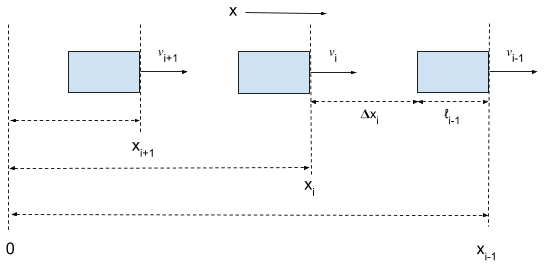
\includegraphics[width=3.75 in]{carLane.png}}
\caption{Line of vehicles in a straight lane.}
\label{fig1}
\end{figure}

\subsection{Variables}
\begin{itemize}
\item Relative distance: The relative distance $\Delta x_i$ for vehicle $i$ is the distance between the front bumper of vehicle $i$ and the back bumper of vehicle $i-1$. That is,
\begin{eqnarray}
\Delta x_i = x_{i-1}-x_i-l_{i-1},
\end{eqnarray}
where $x_{i-1}$ is the position of the front bumper of vehicle $i-1$, $x_i$ is the position of the front bumper of vehicle $i$, and $l_{i-1}$ is the length of vehicle $i-1$.
\item Relative velocity: The relative velocity $\Delta v_i$ for vehicle $i$ is the velocity difference between vehicle $i-1$ and vehicle $i$. That is,
\begin{eqnarray}
\Delta v_i=v_{i-1}-v_i,
\end{eqnarray}
where $v_{i-1}$ is the velocity of vehicle $i-1$ and $v_i$ is the velocity of vehicle $i$.
\item Reference velocity: Also known as the desired velocity or optimal velocity, the reference velocity $r$ is the velocity at which the autonomous vehicle desires to travel. It is typically the average velocity over the length of a traffic wave, and is found by dividing the total distance traveled by a vehicle in front of the AV by the time. That is,
\begin{eqnarray}
r={d_{total}\over t_{total}}
\end{eqnarray}
\item Spacing error: The spacing error $\epsilon_i$ is the difference between the desired relative distance and the actual relative distance, giving,
\begin{eqnarray}
\epsilon_i = \Delta x_{i des}-\Delta x_i.
\end{eqnarray}
\end{itemize}

\subsection{Definitions}
\begin{itemize}
\item Safe: A scenario is safe if at all times for every vehicle $i$ such that $1<i\leq n$, then $\Delta x_i>0$ m. This means that the relative distance will always be greater than 0 for every vehicle.
\item Individual vehicle stable: A velocity control law is considered to be individual vehicle stable if the spacing error of the AV approaches 0 with time if the lead vehicle travels at a constant velocity.
\item String stable: When a lead vehicle accelerates or decelerates in front of an individual vehicle stable AV, the spacing error will momentarily be nonzero. Suppose there is an infinite line of autonomous vehicles with one lead vehicle in front. The velocity control law is considered to be string stable if, during acceleration or deceleration of the lead vehicle, the spacing error decreases with each successive vehicle as they react to the change in velocity \cite{Rajamani}. Additionally, all spacing errors must be in the same direction, either all negative or all positive. INCLUDE FURTHER DESCRIPTIONS OF STRING STABLE VS UNSTABLE GRAPHS
\end{itemize}

\subsection{Infrastructure}
The FollowerStopper velocity controller is first modeled in Simulink and then used in conjunction with ROS to test in the physics-based simulation engine, Gazebo. After demonstrating success in Gazebo, the velocity controller is implemented onto the Cognitive and Autonomous Test (CAT) Vehicle at the University of Arizona using a hardware in the loop (HIL) configuration as described in \cite{Bhadani}.

\hspace{0.01 in}The CAT Vehicle is a modified Ford Hybrid Escape with a SICK LMS 291 Front Laser Rangefinder, a Velodyne HDL-64E S2 LiDAR, two Pointgrey Firefly MV FFMV-03M2C cameras, and a Novatel VPS/IMU. The FollowerStopper velocity controller uses distance data from the LiDAR to determine the relative distance to the car in front $\Delta x_i$. Using the relative distance data, the AV can determine the relative velocity \cite{Real-time}. Assuming that the AV knows its own velocity at all times, it can use the relative velocity data to determine the velocity of the lead vehicle.

\hspace{0.01 in}The delay $\delta$ of the system is of supreme importance because at high speeds, if the vehicle needs to stop, the vehicle can still travel a considerable distance before receiving the stopping command and implementing the command. Contributions to the delay include the LiDAR sensor delay (0.133 s), the moving average filter delay ($\rm {10\ moving\ steps\over 2}(0.01{s\over step})$), and a fixed delay (1.0 s) due to friction, actuator dynamics, controller update rate, etc. From \cite{Real-time}, considering that the position sampling frequency $F_s$ and velocity sampling frequency $F_v$ are both 75 Hz,

\begin{eqnarray*}
\delta &=& {\delta_f F_s \over F_v}+\delta_r = \delta_f +\delta_r \\
&=& 0.133+{10\over 2}(0.01)+1\\
&=& 1.183 \rm\ s
\end{eqnarray*}

where $\delta_f$ is the delay of the filtered LiDAR data and $\delta_r$ is a fixed delay. To be account for safety, the models developed in Simulink assumed a delay of $\delta = 2.0$ s.



%%%%%%%%%%%%%%%%%%%%%%%%%%%%%%%%%%%%%%%%%%%%%%%%%%%%%%%
%%%%%%%%%%%%%%%%%%%%%%%%%%%%%%%%%%%%%%%%%%%%%%%%%%%%%%%
%%%%%%%%%%%%%%%%%%%%%%%%%%%%%%%%%%%%%%%%%%%%%%%%%%%%%%%



\section{Parameters}
In the development of the FollowerStopper controller, several parameters are often used. They are grouped here to allow for easy reference. Some of the parameters involve acceleration due to gravity, which will be taken as $G=9.80665 {m\over s^2}$ for our purposes. In choosing the parameters, safety is the priority. If safety is not a concern, keeping a small distance between the AV and the lead is desirable in order to accommodate for a higher density of cars on the road and to prevent lane changes of human drivers in front of the AV. Table 1 at the end of the section summarizes the findings.
 
\subsection{Minimum relative distance, $\psi$}
Minimum relative distance refers to the minimum acceptable distance between the AV and the lead. While stopped, it is expected that $\Delta x= \psi$. We chose an arbitrary value of $\psi=1$ because we thought that if the AV was any closer to the lead, the passengers of the AV might be uncomfortable because they do not have control of the car. 

\subsection{Comfortable acceleration, $a_{cmft}$}
The comfortable acceleration limits the maximum acceleration of the AV. When the reference velocity increases, the AV will not immediately travel at the reference velocity, but will increase its velocity at an acceleration of $a_{cmft}$. Particularly in congested traffic conditions, it is undesirable for the AV to have jerky velocity changes. Though it is essential to safety to leave the deceleration of the AV unrestrained, limiting the acceleration will provide for greater passenger comfort and expectability. {comfortable acceleration} details comfortable accelerations in the range of $0.11G$ to $0.15G$ for public mass transportation systems. Because passengers will be much less affected by a car's acceleration due to comfortable seating and expectability than a public mass transport acceleration, we chose $0.15G$ a reasonable value.

\subsection{Comfortable deceleration, $a_{dcmft}$}
The comfortable deceleration defines the maximum amount by which the reference velocity can change. In cases where the reference velocity drops to a much lower value, it is not required for the AV to immediately travel at that value in order to remain safe. $a_{dcmft}$ ensures a smooth transition when safety is not of concern. {comfortable acceleration} details $0.266G$ as a deceleration that is comfortable to passengers and is preferred by a driver.

\subsection{Maximum deceleration, $a_{dmax}$}
The maximum deceleration refers to the maximum possible deceleration of the AV. Five different websites \cite{max decel 1,max decel 2,max decel 3, max decel 4, max decel 5} listed different maximum deceleration data for the Ford Escape Hybrid, which is the vehicle under consideration. Every piece of data was based off of an experiment where the vehicle would travel at a constant velocity before braking as hard as possible, and then reporting the stopping distance. For safety purposes, the deceleration with the lowest absolute value was chosen as the maximum deceleration for the Ford Escape Hybrid, that is $-7.66{m\over s^2}$ \cite{max decel 3}. If the maximum deceleration of the AV is not known, \cite{Fambro} details $-3.99{m\over s^2}$ as the maximum deceleration of a passenger car traveling on wet pavement. This can be used if a more accurate estimation cannot be found.

\subsection{Deceleration ratio, $k$}
The deceleration ratio is the ratio between the maximum deceleration of the lead vehicle and the maximum deceleration of the AV. For FollowerStopper to be safe, as is shown in the next section, there must be some knowledge of how the lead and AV accelerations relate. A deceleration ratio less than unity, that is $k<1$, means that the AV can decelerate to a stop faster than the lead, meaning that it can travel closer than normal to the lead and still be safe. A deceleration ratio greater than unity, that is $k>1$, means that the lead can decelerate to a stop faster than the AV, meaning that the AV must follow at a greater relative distance in order to have a greater stopping distance. To be safe, we must assume that the lead vehicle can decelerate as fast as physically possible. From section A of the Appendix, the deceleration of a vehicle is $a=-G\mu$, where $\mu$ is the coefficient of friction. \cite{road conditions} concludes that the maximum tire-road friction coefficient in normal driving on a dry road is $\mu_{max}=1$, so the maximum deceleration of the lead vehicle is $-G$.

\begin{table}[htbp]
\caption{FollowerStopper Parameters}
\begin{center}
\begin{tabular}{|c|c|c|c|}
\hline
\textbf{Name} & \textbf{Symbol} & \textbf{Calculation} & \textbf{Value} \\
\hline
					&				&						&					\\
minimum relative distance	&	$\psi$		&	---					&	1				\\
					&				&						&					\\
comfortable acceleration	&	$a_{cmft}$	&	$0.15\cdot G$			&	1.47$m\over s^2$	\\
					&				&						&					\\
comfortable deceleration	&	$a_{dcmft}$	&	$-0.266\cdot G$		&	-2.61$m\over s^2$	\\
					&				&						&					\\
maximum deceleration	&	$a_{dmax}$	&	---					&	-3.99$m\over s^2$	\\
(general)				&				&						&					\\
deceleration ratio		&	$k$			&	$-G\over a_{dmax}$		&	2.46				\\
(general)				&				&						&					\\
maximum deceleration	&	$a_{dmax}$	&	---					&	-7.66$m\over s^2$	\\
(Ford Escape Hybrid)	&				&						&					\\
deceleration ratio		&	$k$			&	$-G\over a_{dmax}$		&	1.28				\\
(Ford Escape Hybrid)	&				&						&					\\

\hline
\end{tabular}
\label{tab1}
\end{center}
\end{table}



%%%%%%%%%%%%%%%%%%%%%%%%%%%%%%%%%%%%%%%%%%%%%%%%%%%%%%%
%%%%%%%%%%%%%%%%%%%%%%%%%%%%%%%%%%%%%%%%%%%%%%%%%%%%%%%
%%%%%%%%%%%%%%%%%%%%%%%%%%%%%%%%%%%%%%%%%%%%%%%%%%%%%%%



\section{FollowerStopper Description}

\subsection{Classification}
The premise of FollowerStopper is to command exactly the reference velocity $r$ whenever safe because this is the velocity that could dissipate already formed traffic jams and could prevent new traffic jams from forming. If $r>v_{lead}$ and the AV is getting close to the lead, FollowerStopper will command a lower velocity $v_{cmd}$ whenever safety requires, based on the AV's velocity, relative velocity to the lead vehicle, and relative distance to the lead vehicle. Assuming that the two cars start out far enough apart, there are three relative velocity regions.
\begin{enumerate}
\item $v_{lead} > r$: $v_{cmd}=r$ because the AV will not catch up to the lead
\item $v_{lead} = r$: $v_{cmd}=r$ because the AV will not catch up to the lead
\item $v_{lead}<r$: $v_{cmd}\leq r$ because if the AV is far enough away, it can continue to travel at $r$. Once the AV gets within a specified distance $\Delta x \leq \xi_3$ then it must travel less than $r$ in order to prevent a collision. This distance should take into account that hard braking is a contributing factor to traffic jams, so the AV should begin slowing down well in advance of a crash in order to be able to decelerate at a comfortable level of deceleration $a_{dcmft}$.
\end{enumerate}

The Follower Stopper controller from \cite{Real-time} is reproduced below. 
\begin{eqnarray}
v_{cmd} &=& \begin{dcases}
        0 								& \Delta x\leq \xi_1 \\
        v_{lead}^*{\Delta x-\xi_1\over\xi_2-\xi_1} 			& \xi_1< \Delta x\leq \xi_2 \\
        v_{lead}^*+(r-v){\Delta x-\xi_2\over\xi_3-\xi_2}			& \xi_2< \Delta x\leq \xi_3 \\
        r 								& \xi_3< \Delta x \\
    \end{dcases}
\end{eqnarray}
\begin{eqnarray}
\xi_j(\Delta v)	&=& \omega_j + {1\over 2\alpha_j}(\Delta v^*)^2 \ \ {\rm for \ \ j=1, 2, 3}
\end{eqnarray}
where $v^*_{lead} = min(max(v_{lead}, 0), r)$. $r$ is the reference velocity as taken from the output of smoothUpParams and $v_{cmd}$ is the command velocity that is sent to the AV. The $\omega_j$ and $\alpha_j$ values in the equation for $\xi_j$ are distance and deceleration parameters, respectively, and $\Delta v^*=min(\Delta v, 0)$. \cite{Real-time} suggests for future work to optimize the distance and deceleration parameters, which were previously set to $\omega_1=4.5$ m, $\omega_2=5.25$ m, $\omega_3=6.0$ m, $\alpha_1=1.5 {\rm {m\over s^2}}$, $\alpha_2=1.0 {\rm {m\over s^2}}$, and $\alpha_3=0.5 {\rm {m\over s^2}}$. The following sections will seek to accomplish this task of finding the ideal $\xi_j$ values.

\subsection{SmoothUpParams}
Theoretically, the reference velocity will be given to the AV by means of a roadside controller which takes traffic data and determines the optimal constant velocity. The function SmoothUpParams edits the reference velocity once the AV receives it but before it is used by FollowerStopper in order to prevent harsh and unnecessary acceleration or deceleration. SmoothUpParams is a function of the new reference velocity $r$, the autonomous vehicle velocity $v_{AV}$, the maximum comfortable acceleration for the autonomous vehicle $a_{cmft}$, and the maximum comfortable deceleration for the autonomous vehicle $a_{dcmft}$. Using these inputs, SmoothUpParams edits the reference velocity so that it is a reasonable value when it is sent to the FollowerStopper controller. Suppose, for example, the speed limit were to change from 10 m/s to 15 m/s and no car was in front of the AV. FollowerStopper would command the AV to travel at the reference velocity of 15 m/s immediately, but this will result in a large acceleration. SmoothUpParams will cause the reference velocity to increase at a slow rate so that FollowerStopper can still command the reference velocity, but it will not result in a large acceleration.

\subsection{Designing $\xi_1$ for safety}
According to FollowerStopper, if $\Delta x \leq \xi_1$, then $v_{cmd}=0$. That is, if the relative distance between the AV and the lead is less than or equal to $\xi_1$, the AV should brake as hard as possible or remain stopped if already at a stop. The AV will recognize that it should emergency brake at $\Delta x=\xi_1$, but the actual braking will not initiate until $\delta$ seconds after $\Delta x=\xi_1$ due to the system delay. To prove that FollowerStopper is safe, we simply need to show that if $\Delta x = \xi_1$, braking as hard as possible after a delay of $\delta$ seconds will never result in a crash. This assumes that no unexpected obstacle comes between the AV and the lead. The metric is computed as:
\begin{dmath}
\xi_1 = \psi +\Delta v^{**}+v_{AV}(1-{a_{cmft}\over a_{dmax}})\delta+{a_{cmft}\over 2}(1-{a_{cmft}\over a_{dmax}})\delta^2
\end{dmath}
where $\Delta v^{**} = max(0,{1\over 2ka_{dmax}}(v_{lead}^2-kv_{AV}^2))$. The derivation can be found in the Appendix.

\subsection{Designing $\xi_2$ for string stability}
When $v_{AV}>v_{lead}$, the relative distance $\Delta x$ will decrease as the AV approaches the lead. When $\Delta x$ drops below a certain threshold in such a situation, FollowerStopper is designed to incrementally command a smaller velocity $v_{cmd}<v_{AV}$ until the velocity of the AV is equal to the velocity of the lead $v_{cmd}=v_{lead}$. Once $v_{AV}=v_{lead}$, the AV will maintain the string stable distance $\Delta x=\xi_2$. If the relative distance drops below this equilibrium distance, that is $\Delta x<\xi_2$, the velocity of the AV will decrease below $v_{lead}$ in an attempt to recover this distance. The second line of the piecewise FollowerStopper controller in equation 5 demonstrates this concept.

 If the distance is greater than the equilibrium distance, that is $\Delta x>\xi_2$, the velocity of the AV will increase in an attempt to recover this distance unless $v_{lead}$ exceeds the reference velocity, at which point $v_{cmd}=r$. Therefore, the AV will spend the majority of its functioning at or above the distance $\xi_2$. It is important, then, that $\xi_2$ is a string stable distance. According to \cite{Rajamani}, string stability is maintained when the time-gap $h$ between two cars is such that $h\geq2\tau$, where $\tau$ is the time constant of any lags in tracking the command velocity, or in other words, it is the delay of the system $\delta$. Additionally to maintaining a time-gap greater than $2\delta$, it is necessary that $\xi_2>\xi_1$. With this knowledge the metric is computed as: 
 \begin{dmath}
 \xi_2 = \xi_1 + 2v_{AV}\delta
 \end{dmath}

\subsection{Designing $\xi_3$ for comfort}
If $\Delta x>\xi_3$, then $v_{cmd}=r$. Once $\Delta x\leq \xi_3$, the AV will begin a comfortable deceleration before reaching the distance $\xi_2$ that it wants to maintain while $v_{lead}<r$. In order to preserve an equal spacing between all of the relative distance parameters $\xi_3$, $\xi_2$, and $\xi_1$, we design FollowerStopper such that $\xi_2$ is the average of $\xi_1$ and $\xi_3$. A brief amount of algebra reveals the calculation for $\xi_3$. The metric is computed as:
\begin{eqnarray}
\xi_3 = 2\xi_2-\xi_1
\end{eqnarray}

\subsection{Further considerations}
FollowerStopper is designed such that the AV will not accelerate faster than $a_{cmft}$ and will not decelerate faster than $a_{dcmft}$ while $\Delta x > \xi_1$. If, however, $\Delta x\leq \xi_1$, then the AV will decelerate at its maximum possible deceleration $a_{dmax}$. The same concept is implemented in SmoothUpParams. When receiving a new reference velocity, FollowerStopper will edit the reference to increase or decrease from the old to the new reference velocity at an acceleration and deceleration of $a_{cmft}$ and $a_{dcmft}$, respectively.



%%%%%%%%%%%%%%%%%%%%%%%%%%%%%%%%%%%%%%%%%%%%%%%%%%%%%%%
%%%%%%%%%%%%%%%%%%%%%%%%%%%%%%%%%%%%%%%%%%%%%%%%%%%%%%%
%%%%%%%%%%%%%%%%%%%%%%%%%%%%%%%%%%%%%%%%%%%%%%%%%%%%%%%



%\section{Human car-following models}
%
%\subsection{Human Follower 1}
%Demonstrate safety and string instability
%
%\subsection{Human Follower 2}
%Demonstrate safety and string instability



%%%%%%%%%%%%%%%%%%%%%%%%%%%%%%%%%%%%%%%%%%%%%%%%%%%%%%%
%%%%%%%%%%%%%%%%%%%%%%%%%%%%%%%%%%%%%%%%%%%%%%%%%%%%%%%
%%%%%%%%%%%%%%%%%%%%%%%%%%%%%%%%%%%%%%%%%%%%%%%%%%%%%%%



\section{Simulink Verification}

\subsection{Safety flaws of the previous version of FollowerStopper}

\subsection{Safety verification of the current FollowerStopper}

\subsection{String stability verification}



%%%%%%%%%%%%%%%%%%%%%%%%%%%%%%%%%%%%%%%%%%%%%%%%%%%%%%%
%%%%%%%%%%%%%%%%%%%%%%%%%%%%%%%%%%%%%%%%%%%%%%%%%%%%%%%
%%%%%%%%%%%%%%%%%%%%%%%%%%%%%%%%%%%%%%%%%%%%%%%%%%%%%%%



\section{Results}

\subsection{Gazebo interface}

\subsection{CAT Vehicle testing}



%%%%%%%%%%%%%%%%%%%%%%%%%%%%%%%%%%%%%%%%%%%%%%%%%%%%%%%
%%%%%%%%%%%%%%%%%%%%%%%%%%%%%%%%%%%%%%%%%%%%%%%%%%%%%%%
%%%%%%%%%%%%%%%%%%%%%%%%%%%%%%%%%%%%%%%%%%%%%%%%%%%%%%%



\section{Conclusion}

\subsection{Further work}
Deceleration profile is not constant, especially during emergency braking \cite{Akhilesh}

Adjusting $a_{dmax}$ and $k$ based on the road conditions \cite{road conditions}, the type of car in front, and the quality of the tires in the AV \cite{road conditions}

\subsection{CAT Vehicle testing}



%%%%%%%%%%%%%%%%%%%%%%%%%%%%%%%%%%%%%%%%%%%%%%%%%%%%%%%
%%%%%%%%%%%%%%%%%%%%%%%%%%%%%%%%%%%%%%%%%%%%%%%%%%%%%%%
%%%%%%%%%%%%%%%%%%%%%%%%%%%%%%%%%%%%%%%%%%%%%%%%%%%%%%%
%%%%%%%%%%%%%%%%%%%%%%%%%%%%%%%%%%%%%%%%%%%%%%%%%%%%%%%
%%%%%%%%%%%%%%%%%%%%%%%%%%%%%%%%%%%%%%%%%%%%%%%%%%%%%%%
%%%%%%%%%%%%%%%%%%%%%%%%%%%%%%%%%%%%%%%%%%%%%%%%%%%%%%%



\begin{thebibliography}{00}
\bibitem{Sugiyama} Y. Sugiyama et al, ?Traffic jams without bottlenecks?experimental evidence for the physical mechanism of the formation of a jam,? New Journal of Physics, vol. 10, March 2008.

\bibitem{Stern} R. E. Stern, S. Cui, M. L. Monachec R. Bhadani, M. Bunting, M. Churchill, N. Hamilton, R. Haulcy, H. Pohlmann, F. Wu, B. Piccoli, B. Seibold, J. Sprinkle, D. B. Work, ?Dissipation of stop-and-go waves via control of autonomous vehicles: Field experiments,? Transportation Research Part C: Emerging Technologies, vol. 89, pp. 208--221, April 2018

\bibitem{Rajamani} Vehicle Dynamics and Control

\bibitem{Litman} Autonomous vehicle implementation predictions

\bibitem{Bhadani} The cat vehicle testbed: a simulator with hardware in the loop for autonomous vehicle applications

\bibitem{Real-time} Real-time distance estimation and filtering of vehicle headways for smoothing of traffic waves

\bibitem{Supervisory} Dissipation of Emergent Traffic Waves in Stop-and-Go Traffic Using a Supervisory Controller

\bibitem{comfortable acceleration} Hoberock, Lawrence L. "A survey of longitudinal acceleration comfort studies in ground transportation vehicles." Journal of Dynamic Systems, Measurement, and Control 99.2 (1977): 76-84. 
%%%%%BibTex: https://scholar.google.com/scholarhl=en&as_sdt=0%2C3&q=A+SURVEY+OF+LONGITUDINAL+ACCELERATION+COMFORT+STUDIES+IN+GROUND+TRANSPORTATION+VEHICLES+&btnG=

\bibitem{max decel 1}"Escape Hybrid." Carsort, carsort.com/cars/Ford-Escape-Hybrid.

\bibitem{max decel 2}Motortrend.com. 2012 Ford Escape Reviews - Research Escape Prices \& Specs.? MotorTrend, Motor Trend, 1 Apr. 2019, www.motortrend.com/cars/ford/escape/2012/.

\bibitem{max decel 3}"Used 2012 Ford Escape Hybrid Hybrid Review." Edmunds.com, www.edmunds.com/ford/escape/2012/hybrid/st-101387395/review/.

\bibitem{max decel 4}Vanderwerp, Dave. "Ford Escape Hybrid 4WD." Car and Driver, 8 Mar. 2019, www.caranddriver.com/reviews/a15132014/ford-escape-hybrid-4wd-road-test-hybrid-operation-page-1/.

\bibitem{max decel 5}"Vehicle Test Book." Michigan.gov, 2007, www.michigan.gov/documents/msp/VehicleEvaluation2007_MSP-SpecialDesigned_182664_7.pdf.

\bibitem{Fambro} Fambro, D. B., K. Fitzpatrick, and R. J. Koppa. "NCHRP report 400: Determination of stopping sight distances." TRB, National Research Council, Washington, DC (1997). 
%BibTex link: https://scholar.google.com/scholar?hl=en&as_sdt=0%2C3&q=NCHRP+Report+400%2C+Determination+of+Stopping+Sight+Distances&btnG= 

\bibitem{road conditions} Muller, Steffen, Michael Uchanski, and Karl Hedrick. "Estimation of the maximum tire-road friction coefficient." Journal of dynamic systems, measurement, and control 125.4 (2003): 607-617. 
%BibTex: https://scholar.google.com/scholar?hl=en&as_sdt=0%2C3&q=Estimation+of+the+Maximum+Tire-Road+Friction+Coefficient&btnG=

\bibitem{Akhilesh}Maurya, Akhilesh Kumar, and Prashant Shridhar Bokare. "STUDY OF DECELERATION BEHAVIOUR OF DIFFERENT VEHICLE TYPES." International Journal for Traffic \& Transport Engineering 2.3 (2012). 
%BibTex link: https://scholar.google.com/scholar?hl=en&as_sdt=0%2C3&q=STUDY+OF+DECELERATION+BEHAVIOUR+OF+DIFFERENT+VEHICLE+TYPES&btnG=


%\bibitem{b1} G. Eason, B. Noble, and I. N. Sneddon, ``On certain integrals of Lipschitz-Hankel type involving products of Bessel functions,'' Phil. Trans. Roy. Soc. London, vol. A247, pp. 529--551, April 1955.
%\bibitem{b2} J. Clerk Maxwell, A Treatise on Electricity and Magnetism, 3rd ed., vol. 2. Oxford: Clarendon, 1892, pp.68--73.
%\bibitem{b3} I. S. Jacobs and C. P. Bean, ``Fine particles, thin films and exchange anisotropy,'' in Magnetism, vol. III, G. T. Rado and H. Suhl, Eds. New York: Academic, 1963, pp. 271--350.
%\bibitem{b4} K. Elissa, ``Title of paper if known,'' unpublished.
%\bibitem{b5} R. Nicole, ``Title of paper with only first word capitalized,'' J. Name Stand. Abbrev., in press.
%\bibitem{b6} Y. Yorozu, M. Hirano, K. Oka, and Y. Tagawa, ``Electron spectroscopy studies on magneto-optical media and plastic substrate interface,'' IEEE Transl. J. Magn. Japan, vol. 2, pp. 740--741, August 1987 [Digests 9th Annual Conf. Magnetics Japan, p. 301, 1982].
%\bibitem{b7} M. Young, The Technical Writer's Handbook. Mill Valley, CA: University Science, 1989.
\end{thebibliography}
\vspace{12pt}



%%%%%%%%%%%%%%%%%%%%%%%%%%%%%%%%%%%%%%%%%%%%%%%%%%%%%%%
%%%%%%%%%%%%%%%%%%%%%%%%%%%%%%%%%%%%%%%%%%%%%%%%%%%%%%%
%%%%%%%%%%%%%%%%%%%%%%%%%%%%%%%%%%%%%%%%%%%%%%%%%%%%%%%



\onecolumn
\begin{appendix}

\subsection{Determination of the maximum deceleration of the lead vehicle}
To determine the maximum deceleration of the lead vehicle, consider Figure \ref{fig3}.

\begin{figure}[htbp]
\centerline{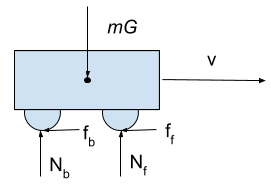
\includegraphics[width=2.00 in]{maxDecel.png}}
\caption{Free-body diagram of a four-wheeled vehicle during deceleration.}
\label{fig3}
\end{figure}

Given the mass, $m$, of the vehicle and acceleration due to gravity, $G$, the normal force acting on the front and back tires can be expressed
\begin{eqnarray*}
mG=N_f+N_b=N.
\end{eqnarray*}
The force of friction is proportional to the normal force by means of the coefficient of friction, $\mu$. Assuming that the force of friction on the front and back tires is equal,
\begin{eqnarray*}
f_f+f_b=N_f\mu+N_b\mu=(N_f+N_b)\mu=N\mu
\end{eqnarray*}
According to Newton's second law, the sum of the forces is proportional to the mass and the acceleration of an object. If we only consider the car's longitudinal direction, or the direction in which it is traveling at velocity, $v$,
\begin{eqnarray*}
\sum F &=& ma \\
-f_f-f_b &=& ma \\
-N\mu &=& ma \\
-mG\mu &=& ma \\
a &=& -G\mu
\end{eqnarray*}




\subsection{Derivation of $\xi_1$}

\begin{figure}[htbp]
\centerline{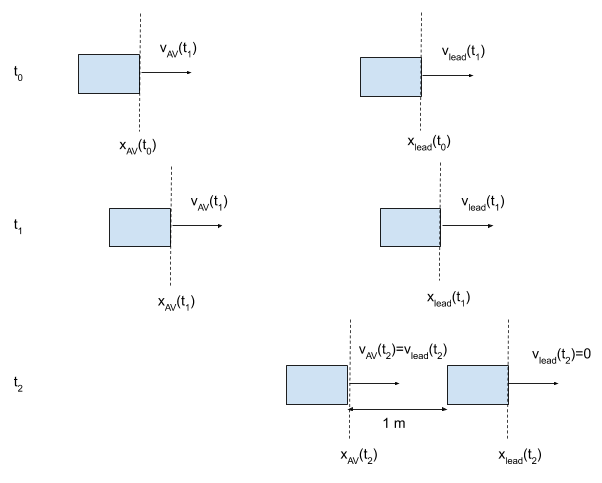
\includegraphics[width=6 in]{xiDerivation.png}}
\caption{Emergency breaking progression.}
\label{fig2}
\end{figure}

Consider Figure \ref{fig2}, depicting two cars at times $t_0$, $t_1$, and $t_2$. $t_0$ is the time at which the relative distance is equal to the emergency breaking distance, that is, $\Delta x(t_0)=\xi_1$. $t_1$ occurs $\delta$ seconds after reaching $\xi_1$, at which point the AV will first be able to react to being within the emergency breaking distance due to the delay. $t_2$ is the time at which both vehicles will be stopped and the AV will be exactly 1 m behind the lead vehicle. The vehicle to the left is the AV and the vehicle to the right is the human-driven lead. All positions and velocities have been labeled as functions of time, and the relative positions and relative velocities at each time can be computed according to the equations in section II.A. First we will consider the motion of the two vehicles from time $t_1$ to time $t_2$. Within this time region in a worst-case scenario, both the AV and lead will constantly decelerate at their maximum decelerations, and in the derivation we will express the lead vehicle maximum deceleration as proportional to the AV maximum deceleration. FIND LEGITIMATE K-VALUE OR THE MAX DECELERATION OF ANY VEHICLE ON THE ROAD. The minimum distance $\Delta x(t_1)$ which can be considered safe will assume that the AV will end up at a relative distance $\Delta x(t_2)= 1$ m from the lead vehicle. The following derivation uses this idea with the equations of motion to derive a value for $\Delta x(t_1)$.

\begin{eqnarray*}
{\rm Equation\ of\ motion:\ } v^2-v_0^2 = 2a\Delta x \\
{\rm Lead\ vehicle:\ } \\
v_{lead}(t_2)^2-v_{lead}(t_1)^2 &=& 2 a_{dmaxLEAD}(x_{lead}(t_2)-x_{lead}(t_1)) \\
{\rm Suppose\ } a_{dmaxLEAD} &=& ka_{dmax} \\
0-v_{lead}(t_1)^2 &=& 2ka_{dmax}x_{lead}(t_2)-2ka_{dmax}x_{lead}(t_1)) \\
2a_{dmax}x_{lead}(t_1) -{v_{lead}(t_1)^2\over k} &=& 2a_{dmax}x_{lead}(t_2) \\
{\rm Autonomous\ vehicle:\ } \\
v_{AV}(t_2)^2-v_{AV}(t_1)^2 &=& 2 a_{dmax}(x_{AV}(t_2)-x_{AV}(t_1)) \\
0-v_{AV}(t_1)^2 &=& 2a_{dmax}(x_{lead}(t_2)-l_{lead}-\psi-x_{AV}(t_1)) \\
2a_{dmax}(l_{lead}+\psi+x_{AV}(t_1))-v_{AV}(t_1)^2 &=& 2a_{dmax}x_{lead}(t_2)\\
{\rm Setting\ the\ equations\ equal:} \\
2a_{dmax}x_{lead}(t_1) -{v_{lead}(t_1)^2\over k} &=& 2a_{dmax}(l_{lead}+\psi+x_{AV}(t_1))-v_{AV}(t_1)^2 \\
2a_{dmax}(x_{lead}(t_1)-x_{AV}(t_1)-l_{lead}) &=& 2a_{dmax}\psi+{v_{lead}(t_1)^2\over k}-v_{AV}(t_1)^2\\
\Delta x(t_1) &=& \psi+{1\over 2a_{dmax}}({v_{lead}(t_1)^2\over k}-v_{AV}(t_1)^2) \\
\end{eqnarray*}

Delay is an essential consideration because if the AV is currently at $\Delta x=\Delta x(t_1)$, it needs to initiate emergency breaking, but it will not do as such until $\delta$ seconds have passed, where $\delta$ is the delay of the system. Consider the time $t_0$ at which point the AV recognizes that it must send an emergency braking command in order to initiate emergency braking at the instant it reaches $t_1$ from the above example. When considering the emergency stopping distance $\xi_1$, we must plan for the worst case scenario. The worst case scenario is that at time $t_0$ the lead car begins to accelerate before coming to an immediate stop because the AV might think that it can begin to accelerate as well. Though from time $t_0$ to time $t_1$ the accelerations might fluctuate, a worst-case scenario would involve maximum acceleration of the AV and maximum deceleration of the lead. FollowerStopper limits the maximum acceleration to be $a_{cmft}$. The following derivation, based off of a derivation in \cite{Real-time}, incorporates the delay to determine what a safe value of $\xi_1$ will equal such that if $\Delta x=\xi_1$, the AV will initiate hard braking at exactly $\Delta x = \Delta x(t_1)$. In this setup, $\xi_1=\Delta x(t_0)$.

\begin{eqnarray*}
{\rm Equation\ of\ motion:\ } x &=& x_0 + v_0t + {1\over 2}at^2 \\
{\rm Distance\ traveled\ during\ delay : \ } \\
x_{lead}(t_1) &=& x_{lead}(t_0)+v_{lead}(t_0)\delta+{1\over 2}a_{lead}(t_0)\delta^2 \\
x_{AV}(t_1) &=& x_{AV}(t_0)+v_{AV}(t_0)\delta+{1\over 2}a_{AV}(t_0)\delta^2
\end{eqnarray*}
Worst-case scenario, $a_{lead}(t_0)=a_{dmaxLEAD}=ka_{dmax}$, $a_{AV}(t_0)=a_{cmft}$
\begin{eqnarray*}
{\rm Incorporating\ relative\ distance:\ } \\
\Delta x(t_1) &=& \Delta x(t_0) + (v_{lead}(t_0)-v_{AV}(t_0))\delta + {1\over 2}(ka_{dmax}-a_{cmft})\delta^2\\
\xi_1 = \Delta x(t_0) &=& \Delta x(t_1) - (v_{lead}(t_0)-v_{AV}(t_0))\delta - {1\over 2}(ka_{dmax}-a_{cmft})\delta^2\\
&=& \psi+{1\over 2a_{dmax}}({v_{lead}(t_1)^2\over k}-v_{AV}(t_1)^2) \\
&& - (v_{lead}(t_0)-v_{AV}(t_0))\delta - {1\over 2}(ka_{dmax}-a_{cmft})\delta^2
\end{eqnarray*}

The above equation for $\xi_1$ guarantees that a crash is impossible and that the AV will never come within 1 meter of the lead, assuming that there are no unexpected obstacles that appear between the AV and the lead. However, when the AV arrives at time $t_0$, it will not know $v_{lead}(t_1)$ or $v_{AV}(t_1)$. Both are best approximated using the equation of motion, $v=v_o+at$, with $a$ set to a safe value. In a worst-case scenario, the $v_{lead}$ will be slower than expected and $v_{AV}$ will be faster than expected. Therefore safe acceleration values will be the same as indicated in the previous derivation. Because all time-dependent values will be expressed at the same time $t_0$, the notation can be dropped, giving
\begin{eqnarray*}
\xi_1 &=& \psi+{1\over 2ka_{dmax}}((v_{lead}+ka_{dmax}\delta)^2-k(v_{AV}+a_{cmft}\delta)^2) - (v_{lead}-v_{AV})\delta - {1\over 2}(ka_{dmax}-a_{cmft})\delta^2 \\
&=& \psi+{1\over 2ka_{dmax}}(v_{lead}^2+2v_{lead}ka_{dmax}\delta+k^2a_{dmax}^2\delta^2-kv_{AV}^2-2kv_{AV}a_{cmft}\delta-ka_{cmft}^2\delta^2) \\
&& -v_{lead}\delta+v_{AV}\delta-{ka_{dmax}\delta^2\over 2}+{a_{cmft}\delta^2\over2} \\
&=& \psi+{v_{lead}^2\over 2ka_{dmax}}+{v_{lead}\delta}+{ka_{dmax}\delta^2 \over 2}-{v_{AV}^2\over 2a_{dmax}}-{v_{AV}a_{cmft}\delta \over a_{dmax}}-{a_{cmft}^2\delta^2\over 2a_{dmax}}-v_{lead}\delta+v_{AV}\delta-{ka_{dmax}\delta^2\over 2}+{a_{cmft}\delta^2\over2} \\
&=& \psi+{1\over 2ka_{dmax}}(v_{lead}^2-kv_{AV}^2)+v_{AV}(1-{a_{cmft}\over a_{dmax}})\delta+{a_{cmft}\over 2}(1-{a_{cmft}\over a_{dmax}})\delta^2.
\end{eqnarray*}

Finally, it must be noted that it is never desirable for $\xi_1$ to drop below $\psi$, the minimum acceptable relative distance. In the above equation for $\xi_1$, the first, third, and fourth terms will always be positive, but the second term could be negative. To assure that $\xi_1$ will remain greater than $\psi$, the second term must be set equal to 0 if it is negative, giving a final solution
\begin{eqnarray*}
\xi_1 &=& \psi+\Delta v^{**}+v_{AV}(1-{a_{cmft}\over a_{dmax}})\delta+{a_{cmft}\over 2}(1-{a_{cmft}\over a_{dmax}})\delta^2 \\
\Delta v^{**} &=& max(0,{1\over 2ka_{dmax}}(v_{lead}^2-kv_{AV}^2)).
\end{eqnarray*}


\end{appendix}

\end{document}
